As we said before, it is most difficut to stop hard radiation (high energy particles), than weak radiation. It is because the mean free path of particles is proportional to their energy so to stop high energy particles large wall thickness would need. Therefore, instead of stopping it, the so-called cosmic vetos are used.

The cosmic veto consists of several complementary detectors, two complementary detectors for each cosmic veto in the case of TRITIUM monitor, with which the hard cosmic events that affect the tritium measurement will be detected and subtracted from the tritium measurement.

As it is shown in Figure \ref{fig:VetoAndPrototype}, the way followed to do that is to place two complementary detectors, called cosmic detectors, one above the TRITIUM cell and the other below it. The distance between both detectors, $34.2~\cm$ for our latest prototype developed, is set by the TRITIUM prototype that has to be placed between both.

\begin{figure}[h]
\centering
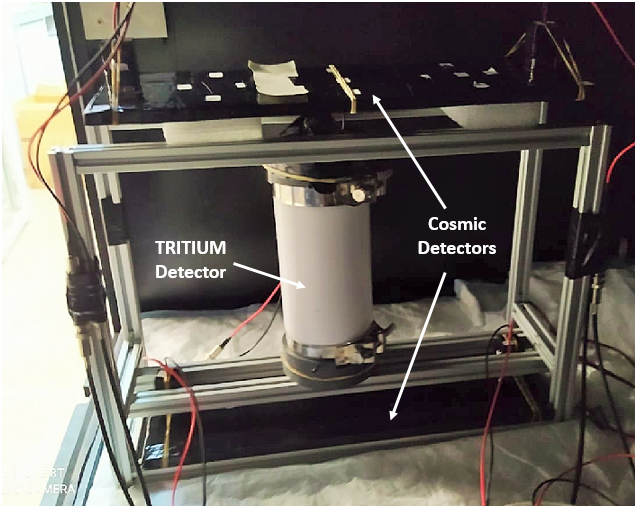
\includegraphics[scale=0.45]{3DesignPrinciples/34BackgroundRejectionSystem/Vetos_y_prototipo.png}
\caption{Cosmic veto and Tritium-IFIC 2 prototype in an aluminum mechanical structure developed by IFIC's mechanical engineering department.\label{fig:VetoAndPrototype}}
\end{figure}

The cosmic veto is placed within the lead shielding so that, the weak radiation doesn't affect them with a false hard cosmic events detected.

A hard cosmic events that affects the tritium measurement will pass through both cosmic detectors at the same time, shown in figure \ref{subfig:RealHardCosmicEvent}. Each cosmic detector will have two photosensors so there are four photosensors in each cosmic veto. Therefore,  to eliminate the hard cosmic events, both cosmic detectors are read out in coincidence with the electron configuration shown in Figure \ref{subfig:ElectronicConfiguraiton4PMT}. Then, the TRITIUM detector is read out in anti-coincidence with the cosmic veto to save the tritium measurement only when there is not any hard cosmic event. 

%In this case, if we have detect a hard cosmic event (time coincidence event in both cosmic detectors), we can be quite sure that it will cross through the tritium detector and, therefore, it will affect to their measurement, as you can see in Figure \ref{subfig:RealHardCosmicEvent}.

It is possible that this hard cosmic event detected in the cosmic veto comes from two different hard cosmic events (one detected in each cosmic detector as shown in Figure \ref{subfig:FakeHardCosmicEvent} but it is practically negligible.

The expected hard cosmic rate at sea level for muons, which is the main contributor of cosmic radiation at this height, is $70~\meter^{-2}\second^{-1}\steradian^{-1}$ \cite{PDG, HardCosmicMuonRate}, that is, approximately, $10^{-2}~\cm^{-2}\second^{-1}\steradian^{-1}$, shown in the cosmic rate plot of Figure \ref{subfig:HardCoscmicRate}. Taking into account that time coincidences are doing with signals whose width is of the order of $10~\nano\second$, the probability of obtaining two different hard cosmic events in temporal coincidence is less than $10^{-9}$ which is insignificant so they are not worth considering.

\begin{figure}[h]
 \centering
  \subfloat[Real hard cosmic event.]{
   \label{subfig:RealHardCosmicEvent}
    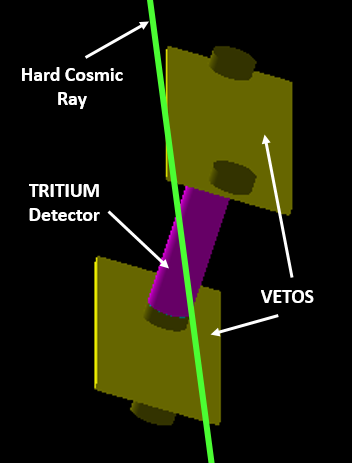
\includegraphics[width=0.25\textwidth]{3DesignPrinciples/34BackgroundRejectionSystem/Real_Event.png}}    
  \subfloat[Fake hard cosmic event.]{
   \label{subfig:FakeHardCosmicEvent}
    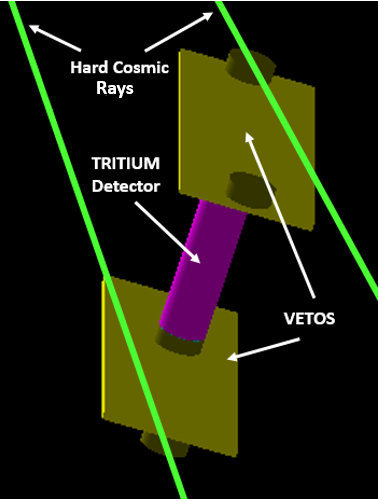
\includegraphics[width=0.25\textwidth]{3DesignPrinciples/34BackgroundRejectionSystem/Fake_Event.png}} 
    \subfloat[Hard cosmic muon rate \cite{HardCosmicMuonRatePlot}.]{
   \label{subfig:HardCoscmicRate}
    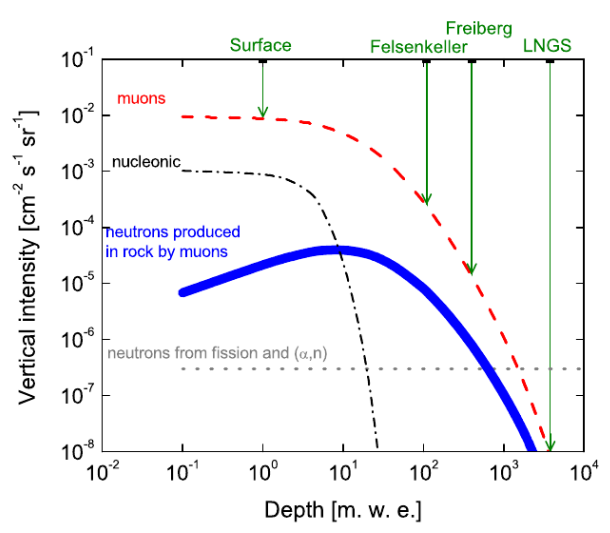
\includegraphics[width=0.42\textwidth]{3DesignPrinciples/34BackgroundRejectionSystem/HardCosmicRate.png}}     
 \caption{Hard cosmic events detected with the cosmic veto of TRITIUM: a) Affecting to the tritium measurement, b) Does not affecting to the tritium measurement. c) Hard cosmic muon rate. }
 \label{fig:HardCosmicEventsSimulation}
\end{figure}

Finally, these individual cosmic detectors on which the cosmic veto is based, consist of a plastic scintillator block from Epic-Crystal \cite{ScintillatorVeto}, whose properties and energy emission spectrum are shown in Table \ref{tab:ParametersScintillatorVeto} and Figure \ref{fig:EmissionEnergySpectrumVeto} respectively.

\begin{table}[]
%%\centering
\begin{center}
\begin{tabular}{|c|c|c|}
%\hline
%Material & Refractive index \\
\hline \hline 
Base material & Polystyrene \\ \hline
Growth method & Polymeric \\ \hline
Density ($\gram/\cm^3$)& 1.05 \\ \hline
Refractive index & 1.58 \\ \hline
Soften temperature ($\degree$) & 75-80 \\ \hline
Light output (Anthracene) & 50-60\% \\ \hline
H/C raito & 1.1 \\ \hline
Emission peak (nm) & 415 (Blue) \\ \hline
Decay Time, (ns) & 2.4 \\ \hline
Hygroscopic & No \\ \hline
\end{tabular}
\caption{Properties of plastic scintillator blocks from Epic-Crystals. \cite{ScintillatorVeto}}
\label{tab:ParametersScintillatorVeto}
\end{center}
\end{table}

\begin{figure}[]
\centering
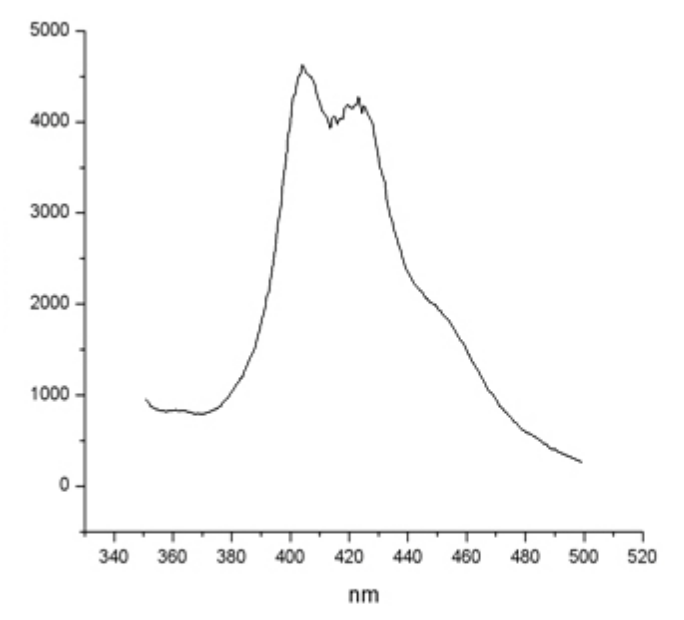
\includegraphics[scale=0.45]{3DesignPrinciples/34BackgroundRejectionSystem/EmissionEnergySpectrumVetos.png}
\caption{Emission energy spectrum of the plastic scintillation used for the cosmic vetos.\label{fig:EmissionEnergySpectrumVeto}~\cite{ScintillatorVeto}}
\end{figure}

It has an emission peak very close to that of the scintillating fibers used, so the same photosensors are used to read out them. The dimensions of the scintillator block are $45~\cm$ long, $17~\cm$ deep and $1~\cm$ of thickness and they are covered by three layers, teflon, aluminum and black tape, shown in Figure \ref{fig:LayersVeto}. These layers has two objectives. On the one hand, they are used to prevent external photons from reaching the scintillator plastic, giving false hard cosmic events and, on the other hand, they are used to prevent the photons generated by the scintillator plastic from escaping before reaching the photosensor, losing real hard cosmic events.

\begin{figure}[h]
 \centering
  \subfloat[Scintillator without coating.]{
   \label{subfig:PlasticScintillatorNoCoating}
    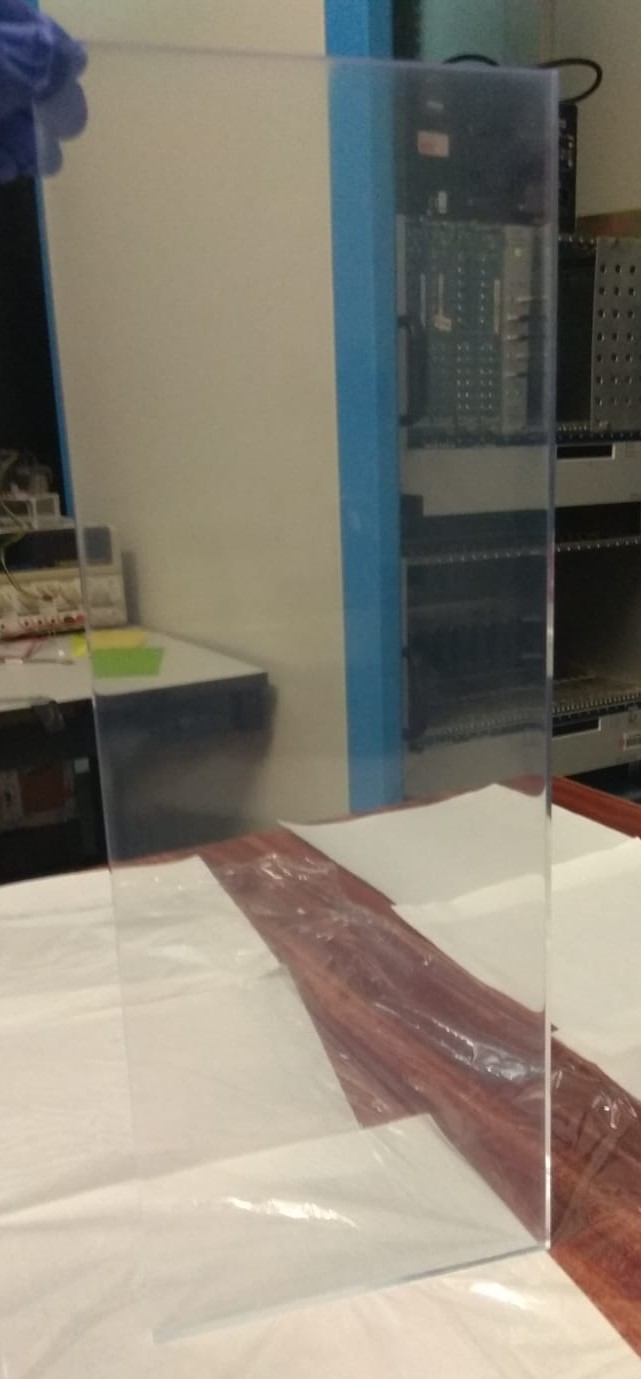
\includegraphics[width=0.23\textwidth]{3DesignPrinciples/34BackgroundRejectionSystem/NoCoating.jpeg}}    
  \subfloat[Teflon coating.]{
   \label{subfig:PlasticScintillatorTeflon}
    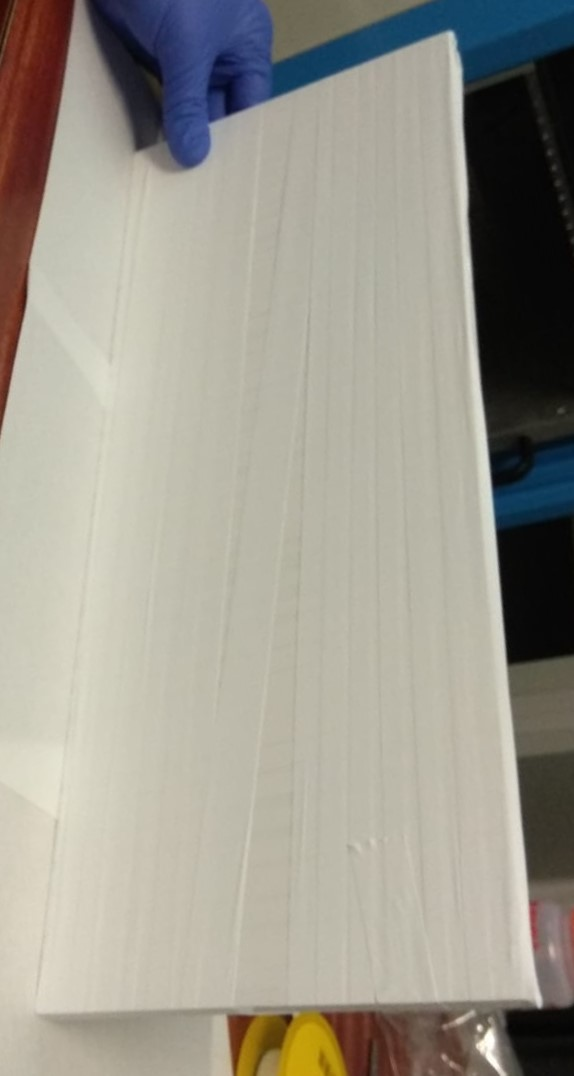
\includegraphics[width=0.23\textwidth]{3DesignPrinciples/34BackgroundRejectionSystem/TeflonCoating.jpeg}}  
  \subfloat[Aluminium coating.]{
   \label{subfig:PlasticScintillatorAluminium}
    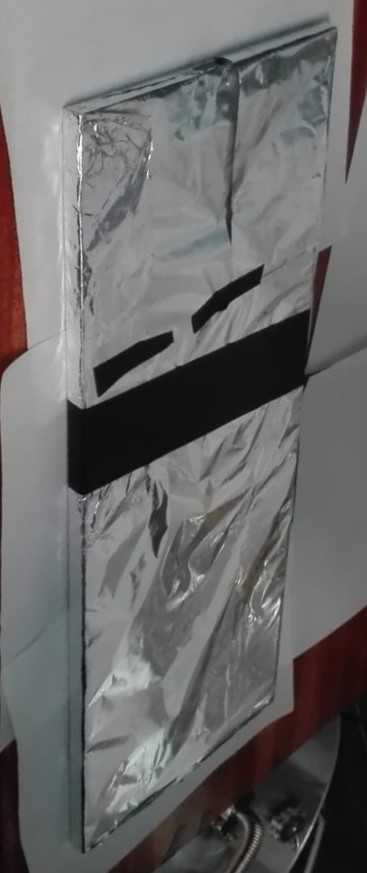
\includegraphics[width=0.23\textwidth]{3DesignPrinciples/34BackgroundRejectionSystem/AluminiumCoating.jpeg}}    
  \subfloat[Black tape coating.]{
   \label{subfig:PlasticScintillatorBlackTape}
    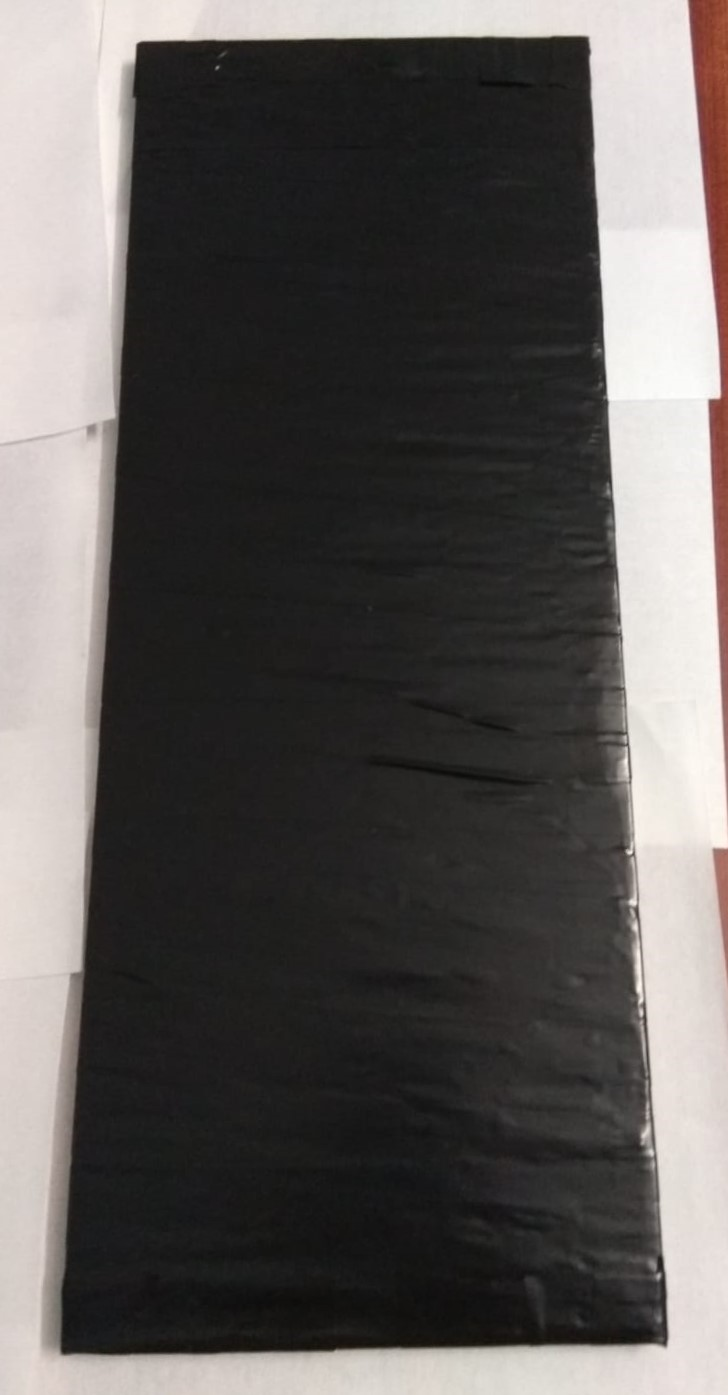
\includegraphics[width=0.23\textwidth]{3DesignPrinciples/34BackgroundRejectionSystem/BlackTapeCoating.jpeg}}
 \caption{Different layers used to cover of the cosmic veto.}
 \label{fig:LayersVeto}
\end{figure}

Two $2.5\cdot{} 2.5 ~\cm^2$ windows are made done in this coating and used to read the photons produced by the plastic scintillator with photosensors.

The expected hard cosmic rate is calculated for our specifically cosmic vetos. The expected hard cosmic rate at sea level is $10^{-2}~\cm^{-2}\second^{-1}\steradian^{-1}$, previously mentioned. Taking into account that, on the one hand, the solid angle of our detectors is $\omega=0.5434$, which has been calculated by integrating above the area of the TRITIUM cosmic veto, and the area of its cosmic veto is $45~\cm \cdot{} 17~\cm=765~\cm^2$, the expected hard cosmic rate on our cosmic vetos should be $2,909~$event$/\second$. It is an important calculation used in experimental measurements to determine the efficiency of the cosmic veto.